\documentclass[conference]{IEEEtran}
\IEEEoverridecommandlockouts
% The preceding line is only needed to identify funding in the first footnote. If that is unneeded, please comment it out.
\usepackage{cite}
\usepackage{amsmath,amssymb,amsfonts}
\usepackage{algorithmic}
\usepackage{graphicx}
\usepackage{textcomp}
\usepackage{xcolor}
\usepackage{color}
\usepackage{url}
\usepackage{gensymb}
\usepackage[paper=a4paper,top=105pt,bottom=54pt,right=37pt,left=54pt]{geometry}% http://ctan.org/pkg/geometry

\def\BibTeX{{\rm B\kern-.05em{\sc i\kern-.025em b}\kern-.08em
    T\kern-.1667em\lower.7ex\hbox{E}\kern-.125emX}}

\hyphenation{op-tical net-works semi-conduc-tor}
\newcommand{\xslnote}[1]{{\bf\color{red}[ #1 -- SHERRY ]}}
\newcommand{\red}[1]{{\bf\color{red}#1}}


\begin{document}


\title{\vspace{17pt} Distributed macroscopic traffic \\ simulation with Open Traffic Models}

\author{\IEEEauthorblockN{Gabriel Gomes}
\IEEEauthorblockA{\textit{Institute of Transportation Studies} \\
\textit{University of California}\\
Berkeley, CA, USA \\
gomes@berkeley.edu}
\and
\IEEEauthorblockN{Juliette Ugirumurera}
\IEEEauthorblockA{\textit{Computational Science Center} \\
\textit{National Renewable Energy Laboratory}\\
Denver, CO, USA \\
jugirumu@nrel.gov}
\and
\IEEEauthorblockN{Xiaoye S. Li}
\IEEEauthorblockA{\textit{Computational Research Division} \\
\textit{Lawrence Berkeley National Laboratory}\\
Berkeley, CA, USA \\
xsli@lbl.gov}
}

\maketitle

\begin{abstract}
This paper presents OTM-MPI, an extension of the Open Traffic Models platform (OTM) for running macroscopic traffic simulations in high-performance computing environments. OTM-MPI represents
the first open-source, distributed-memory, macroscopic
simulation model developed for modern high performance
parallel machines and large networks. Macroscopic simulations are appropriate for studying regional traffic scenarios when aggregate trends are of interest, rather than individual vehicle traces. They are also appropriate for studying the routing behavior of \textit{classes} of vehicles, such as app-informed vehicles. The network partitioning was performed with METIS. Inter-process communication was done with MPI (message-passing interface). Results are provided for two networks: one realistic network which was obtained from Open Street Maps for Chattanooga, TN, and another larger synthetic grid network. The software recorded a speedups of 198x using 256 cores for Chattanooga, and 475x with 1,024 cores for the synthetic network. 

\end{abstract}

\begin{IEEEkeywords}
Traffic simulation, Parallel simulation, Macroscopic traffic simulation, Parallel computing
\end{IEEEkeywords}

\IEEEpeerreviewmaketitle


\section{Introduction}
% Simulation speed is crucial when traffic simulation is used in real-time traffic management or traffic forecasting applications \cite{lee2002framework}.
\IEEEPARstart{R}{ecent} years have seen significant technological changes in transportation with the advent of shared-mobility like Uber and Lift, electric vehicles, and autonomous. There is a need for government agencies and industry to understand the impact of wide-spread adoption of these new technologies on the large-scale transportation system. This in turn requires tools to model the transportation system at the regional scale, requiring large computing and memory resources. Parallel computation and modern supercomputers provide the power and memory to handle such large-scale traffic simulations. They also enable running thousands of parallel simulations that can answer future what-if scenarios.
Traffic simulation developers have adopted parallel computation techniques for traffic simulation of large networks. On a multiprocessor shared-memory computer, parallel simulation takes advantage of the computer's many processors to execute tasks in parallel. In this case, the simulation speed-up is limited by the number of processors on the one computer. On a multiprocessor distributed-memory computer system, parallel simulation can use processors on multiple computers while communicating over a message passing system. This paper describes such an approach for a fluid-based traffic simulation models. We begin by reviewing previous efforts, most of which have focused on vehicle-based (microscopic and mesoscopic) models. 

% We should have a section that show when to use macroscopic simulation and why it is needed at large-scale too. 

\subsection{Related Works}

\begin{table*}[htbp]
\centering
\begin{tabular} { | l | p{25mm} | p{80mm}| } 
	\hline
	\hline
	\textbf{Software} & \textbf{Traffic Model} & \textbf{Parallel Method}\\ \hline
	Paramics \cite{cameron1996paramics} and FastTrans \cite{thulasidasan2009accelerating}    & Microscopic Model & Parallel computation on distributed-memory computer with MPI for inter-core communication \\ \hline
	TRANSIMS \cite{robertson1969transyt}     & Microscopic Model & Parallel computation on distributed-memory computer with MPI and PVM for inter-core communication \\ \hline
	AIMSUN \cite{ferrer1993aimsun2}, SEM-Sim \cite{aydt2013multi} and MEgaffic \cite{osogami2012research}     & Microscopic Model & Multi-threading \\ \hline
	SUMO \cite{behrisch2011sumo}    & Microscopic Model & Multi-threading for routing \\ \hline
	BEAM \cite{aboutBeam}    & Microscopic Model & Akka library \\ \hline
	Dynemo \cite{nokel2002parallel}  & Mesoscopic Model & Network distribution through master-slave parallelization \\ \hline
	Mobiliti \cite{chan2018mobiliti}     & Mesoscopic Model & Parallel discrete event with GASNet \\ \hline
	POLARIS \cite{auld2016polaris}     & Mesoscopic Model & Multi-threading \\ \hline
	\cite{xu2014mesoscopic,song2017supporting}and \cite{strippgen2009multi}     & Microscopic Model & Parallel computation on GPUs \\ \hline
	\cite{chronopoulos1998real}     & Macroscopic Model & Distribution of freeway sections on multiple processes of a nCubes2 distributed-memory parallel computer \\ \hline
	\cite{johnston1999parallelization}     & Macroscopic Model & Distribution of highway segments on multiple processes of a Cray T3W distributed-memory parallel computer \\ \hline
	OTM     & Macroscopic Model & Domain decomposition of network with highway, arterial and local roads. Use MPI for inter-process communication \\ \hline
\end{tabular}
\caption{Softwares for Dynamic User Equilibrium}
\label{tab:softwares}
\end{table*}

%\xslnote{Define micro-, meso- and macro simulations.}

Since Greenshield presented the first traffic model in 1934 \cite{greenshields1934photographic}, three main traffic model categories have emerged: microscopic models, macroscopic models and mesoscopic models. Microscopic models traffic by representing the behavior and interaction of individual vehicles. Macroscopic models describe traffic as a continuum flow with density, flow and speed parameters. Mesoscopic models combine characteristics of macroscopic and microscopic models: traffic movement is represented in aggregate way, while the rules of behavior are modeled per individual vehicles \cite{van2015traffic}. Traffic simulation software tools can also be grouped into microscopic, macroscopic and mesoscopic simulators depending on the model they implement. 

Most prominent traffic simulation software that have parallel computation implementations are microscopic traffic simulators. Parallel Microscopic Simulation (Paramics) \cite{cameron1996paramics} microscopic simulator was implemented on a the T3D parallel computer with Message Passing Interface (MPI) for inter-processor communication. FastTrans \cite{thulasidasan2009accelerating} and TRansportation ANalysis and SIMulation System (TRANSIMS) \cite{nagel2001parallel} microscopic simulators use parallel computation on distributed-memory
%multi-core \xslnote{In 1996, there is no multi-core machine.} 
computer systems by dividing the road network into multiple sub-networks that are distributed among processes running on the multiple computing cores; FastTrans use MPI library to share boundary information among processes, while TRANSIMS can support
both MPI and Parallel Virtual Machine (PVM) communication interface. The Advanced Interactive Microscopic Simulator for Urban and Non-Urban Networks (AIMSUN) \cite{ferrer1993aimsun2}, Scalable Electro-Mobility Simulation (SEM-Sim) \cite{aydt2013multi}, and the IBM Mega Traffic Simulator (MEgaffic) \cite{osogami2012research} implement parallel computation through the multi-threading approach, which enables to run multiple threads in parallel to update simulated agents simultaneously. The Simulation of Urban Mobility (SUMO) microscopic simulator
exploits multi-threading parallel computation for vehicle routing,
but the rest of simulation is single-core \cite{behrisch2011sumo}.
The Behavior, Energy, Autonomy and Mobility (BEAM) simulator \cite{aboutBeam} extends the Multi-Agent Transportation simulator (MATSIM) \cite{horni2016multi}, which is a microscopic traffic simulator. BEAM incorporates parallel computation via the Akka \cite{akka} library, which implements the Actor Model computation \cite{actorModel}. 

 For mesoscopic traffic simulation, N{\"o}kel and Schmidt present a parallel implementation for the Dynemo mesoscopic simulator that uses a master-slave parallelization. The master process initializes the simulation and distributes the network among multiple slave processes. The slave processes calculates the spatial motion of the vehicles on their sub-networks and shares boundary information through PVM communication interface. Mobiliti \cite{chan2018mobiliti} is another mesoscopic traffic simulator that model links as agents and vehicles as events. It uses the parallel discrete event paradigm and a GASNet communication layer to enable parallel computation on high performance computing resources or clusters.The POLARIS mesoscopic simulator \cite{auld2016polaris} exploits parallel computation via multi-threading. References  \cite{xu2014mesoscopic,song2017supporting,strippgen2009multi} present mesoscopic traffic simulation frameworks that take advantage of parallel computation on graphics processing units (GPUs). 

On the other hand, parallel computation has not been applied extensively in macroscopic traffic simulation. Work \cite{chronopoulos1998real} present a parallel implementation of a continuum traffic flow model for freeway modeling on a nCubes2 hypercube distributed-memory parallel computer, where freeway is partitioned into equal segments and assigned to different processors. Each processor sends the calculated density, speed and volume on its segment to processors handling adjacent segments. Similarly, Johnston and Chronolopoulus \cite{johnston1999parallelization} describe a parallelization of lax-momentum traffic model for a highway that divided the highway into equal segments assigned to different processors. The simulation was run on Cray T3E 
%\xslnote{I know about T3D, T3E, but not T3W}
distributed-memory computer system. Though \cite{chronopoulos1998real} and \cite{johnston1999parallelization} use parallel computation for macroscopic traffic simulation on distributed-memory computers, they are focused on freeway simulation. In addition, the performed simulation studies were on small networks (18 to 20 mile freeway) and were executed on older computer systems.

The work we present here is based on the Open Traffic Models simultor. OTM is a full-featured traffic simulator that has in the past been used in single-process environments. OTM is a \textit{hybrid} simulator, in the sense that it incorporates multiple (macroscopic, mesoscopic, and microscopic) models which can be combined arbitrarily on a single network. It also supports multiple road geometries (turn pockets, managed lanes on freeways, etc.), multiple vehicle types, and a variety of traffic control systems (traffic signals, variable speed limits, onboard information systems, etc.). Here we focus on the parallelization of the macroscopic model only. This is both because there are many high quality distributed implementations of vehicle-based models, and because it avoid some of the complexities of asynchronous updates that occur in vehicle-based model.


\section{Methodology}
In this section we begin by describing the methodology for dividing the network. We then describe the inter-process communication. Finally we give a brief description of the macroscopic traffic model. 

\begin{figure*}
\centering
  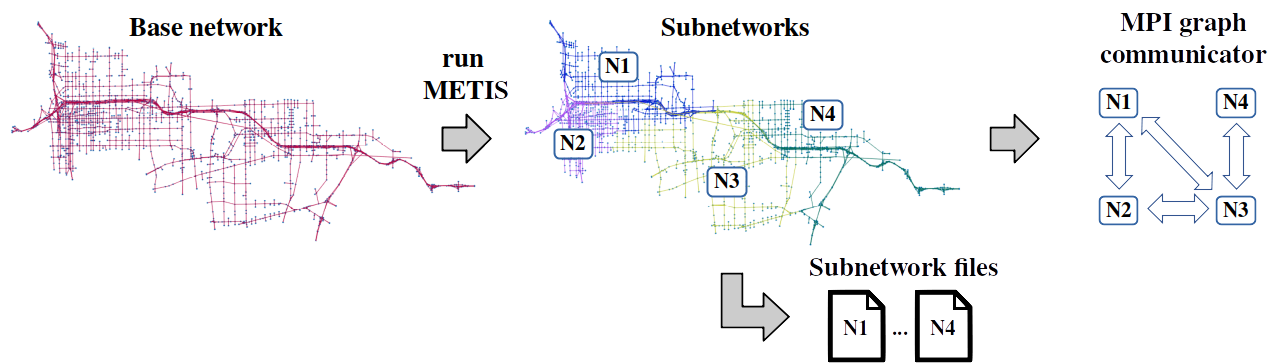
\includegraphics[width=\textwidth]{figs/splitter.png}
  \caption{Network partitioning.}
  \label{fig:partition}
\end{figure*}

\subsection{Network partitioning}
The process of distributing the simulation among $n$ cores is illustrated in Figure~\ref{fig:partition}. The first step is to split the base network into $n$ subnetworks. To obtain these, the set of nodes is divided into non-overlapping sets. Let $\mathcal{N}_i$, $i\in[1\hdots n]$, denote the $i$th subset of nodes. The $i$th subnetwork contains all of the nodes in $\mathcal{N}_i$, as well as all of the links with either start or end node in $\mathcal{N}_i$. 
Links with start node in one subset and end node in another constitute the \textit{overlap} between two subnetworks. An overlap link with start node in $\mathcal{N}_i$ and end node in $\mathcal{N}_j$ is called a \textit{relative source} with respect to subnetwork $j$ and a \textit{relative sink} with respect to subnetwork $i$. The road connections that enter (exit) a relative source (sink) link are called \textit{relative source (sink) road connections} (with respect to a given subnetwork). The implementation utilizes an off-line module that invokes METIS~\cite{kaku:98a} to create the node subsets, and then constructs separate input files for each of the subnetworks. These files contain all of the information (and only that information) that is required to run the given subnetwork as a stand-alone simulation. 

\subsection{Process communication}

The connections between the $n$ subnetworks are encoded in a so-called \textit{metagraph}. This is a graph in which each vertex represents the non-overlapping portions of a subnetwork, and the edges are the relative sources and sinks. Each subnetwork is executed by a separate process. The appropriate MPI communicator for this configuration is the \textit{graph communicator}, which encodes the relations of the metagraph. An all-to-all transmission with a graph communicator exchanges messages amongst neighboring vertices in the metagraph. 

The message passed between two neighboring subnetworks consists of an array of numbers representing the vehicles that travel along all of the relative source and sink road connections that join the two subnetworks. During the initialization phase, the processes construct and exchange decoder maps with each of their neighbors. These map each position in the array to a lane group and state index. This same map is used throughout the entire simulation. The approach is conservative in the sense that the size of the message is fixed, and may contain many zeros at any given time. As is shown in Section~\ref{sec:experiments}, the communication time is a small fraction of the total run time, and hence the potential advantage of using dynamic message sizes is small.

The number of vehicles that travel at each time step over relative road connections (i.e. the flow between subnetworks) is computed by the node model in step 2. The MPI communication step is then inserted between steps 2 and 3. This completes the input and output flow computation for relative sources and sinks. After this, step 3) is executed to compute the downstream link for probabilistically routed vehicles, and then the internal state of all of the lane groups is updated. These steps are identical to their counterparts in the sequential model. Hence the result is not affected by the distribution of the calculation over multiple processes.


\subsection{Traffic modeling}
The full mathematical description of OTM can be found in~\cite{Gomes2019OTM}.
The description provided here omits certain details, but is sufficient to understand the inter-process communication that enables distributed simulation. The model is in the class of \textit{cell transmission} models first introduced by Daganzo in \cite{DaganzoCTM}. Since then there have been many extensions and improvements to the CTM, incorporating multiple lanes, non-triangular fundamental diagrams, etc. The CTM model that is implemented in OTM is adapted to an underlying representation of the road network that can be applied to the different  models in the hybrid simulation environment. As with most traffic simulators, there is a high-level graph (links and nodes) which encodes the connectivity of the road network. Each link (i.e. a segment of road between two junctions) has an internal geometry consisting of multiple lanes, turn pockets, and possibly a managed lane with access gates (in the case of a freeway link). There can also be sensors and control devices within the link. 

The relations between lanes that enter and exit a junction are defined by \textit{road connections}. A road connection indicates which lanes in an upstream link can turn into which other lanes in a downstream link. For example, a road connection may indicate that vehicles must be in the outer two lanes of the freeway in order to reach the off-ramp. The road connections that leave a link are used by the program to aggregate lanes into \textit{lane groups}. All lanes in a lane group access the same set of downstream road connections, and are therefore presumed to travel at similar speeds. In our previous example, the two outer lanes of the freeway constitute a lane group, and the remaining inner lanes are another. 

Vehicles in OTM (whether microscopic, mesoscopic, or macroscopic) are classified according to their \textit{type}. The vehicle type encodes two sets of parameters. First, it determines the vehicle's routing behavior which may be deterministic or probabilistic. Deterministically routed vehicles follow a predetermined sequence of links from their origin to their destination. Probabilistically routed vehicles direct themselves at every junction according to time-varying turning probabilities. The software supports arbitrary numbers of deterministic and probabilistic vehicle types. The second parameter of the vehicle type is a \textit{vehicle class}. The vehicle class encodes any set of parameters that the modeler wishes to prescribe. For example, it can be used to distinguish passenger vehicles from trucks (vehicle size), high-occupancy vehicles from single-occupancy vehicles (lane-usage rules), routing app equipped versus not (access to network information), etc.

In OTM's macroscopic model, each lane group is divided into a sequence of \textit{cells}. The state of each cell is the number of vehicles for each vehicle type and each downstream link. The downstream link of a vehicle is the next link in its route. This is determined in step 3) below for probabilistically routed vehicle types. Vehicles change lanes (ie move laterally between cells in adjacent lane groups) in order to reach a lane group that connects (via road connections) to its downstream link. 

The state update for each cell is executed in multiple steps, listed below. The respective formulas can be found in \cite{Gomes2019OTM}.

\vspace{1em} \noindent \textbf{1) Demand and supply calculations.} The total demand and supply for every cell are computed using the standard formulas of the cell-transmission model for a triangular fundamental diagram. For the last cell in each lane group, the demands are computed for each of the road connections that connect to the respective downstream links. Prior to computing the longitudinal demand, the model executes all lateral movements (lane changes).  

\vspace{1em}\noindent \textbf{2) Inter-link flow calculation.} The flows between links travel along road connections. The \textit{node model} resolves these flows from upstream demands and downstream supplies. The details of the node model can be found in \cite{Gomes2019OTM}. Here it will suffice to state that the output of the node model is a set of \textit{vehicle flux packets} that are delivered along road connections to downstream links. The node model ensures that the downstream links have sufficient available space to accommodate the packets.  

\vspace{1em}\noindent \textbf{3) Probabilistic routing.}
When a node has several outgoing links, probabilistically routed vehicles select which one to take according to given turning probabilities. These probabilities are sampled when the vehicle \textit{enters} the approaching link. This is in contrast with many macroscopic models where turning probabilities are sampled at the node, i.e. when the vehicle \textit{exits} the approaching link. This is done in order to improve the representation of lane changing that occurs upstream of the split.

\vspace{1em} \noindent \textbf{4) State update.} Once all packets have been received and tagged with their next downstream link, then the state of the cells can be updated using the conservation of vehicles. This calculation follows the standard cell transmission model formulas for internal cells. 



\section{Experiments}
\label{sec:experiments}
We ran OTM-MPI on Cori, a Cray XC40 supercomputer at NERSC~\cite{Cori}. Each of Cray's processing nodes has two sockets, each with a 16-core Intel\textcopyright~Xeon\texttrademark~Processor E5-2698 v3 (``Haswell'') at 2.3 GHz and 128 GB of RAM memory. This is a very modern parallel computer, taking advantage of recent advances in parallel computing technology. We report here two experiments; one with a model of Chattanooga, TN, and another with a large synthetic network. 

\subsection{Experiments with the Chattanooga network}

OTM includes a module for extracting networks from Open Street Maps \cite{otmtools,haklay2008openstreetmap}. This module was used to construct a model of  Chattanooga, Tennessee (see Figure~\ref{fig:chattanooga}). The goal of this experiment is to demonstrate the improvements in computation time that can be achieved by distributing computation over many processes for a realistic traffic network topology. Traffic performance metrics were not collected, nor was any effort made to reproduce the demand or routing characteristics of Chattanooga. The network has 32,260 nodes, 38,440 links, and contains 248 source links. Each of these was supplied with a large congestion-inducing demand of 2,000 vph per lane. We conducted 9 runs. In each, the number of parallel processes used was doubled, starting from a single process and up to 256 processes. Each trial was initialized with an empty network and was advanced 10,000 time steps. Figure \ref{fig:chattanooga_plots} shows the results of the simulation performance. 

\begin{figure}[!ht]
\centering
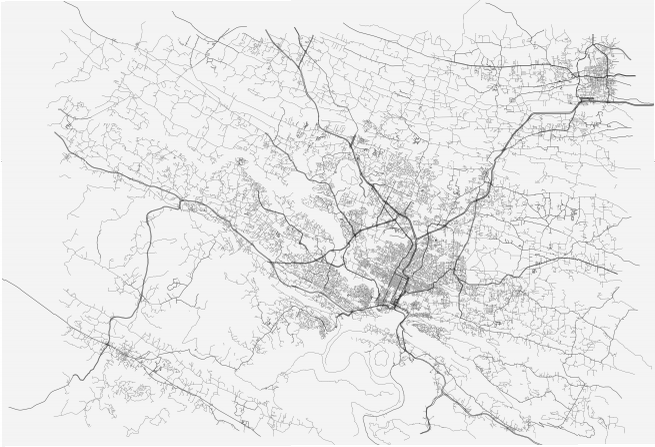
\includegraphics[width=\columnwidth]{figs/chattanooga.png}
\caption{OTM model of the Chattanooga, TN. Bounding box: 34.753\degree north, 35.445\degree south, -85.506\degree east, -84.902\degree west. This model has 32,260 nodes and 38,440 links. }
\label{fig:chattanooga}
\end{figure}

In all of the subplots of the figure, the x-axis is the number of processes involved in the simulation ($n$), represented in base-2 logarithmic scale. The first plot shows that, as expected, the average size of the subnetworks generated by METIS is inversely proportional to the number of processes. The second subplot shows the setup time of the program. This includes the network load time and the time taken to create the MPI communicator and distribute the message decoders. Notice that this load time reaches a minimum and increases slightly for 256 processes. This is because, although the subnetworks are smaller, the complexity of the metagraph and decoders increases and becomes significant for $n=256$. 
\begin{figure}[!ht]
\centering
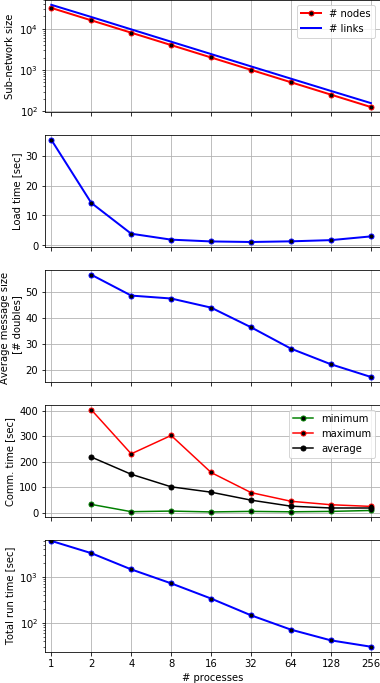
\includegraphics[width=\columnwidth]{figs/chattanooga_plots.png}
\caption{Simulation results for the Chattanooga network.}
\label{fig:chattanooga_plots}
\end{figure}

The third plot shows the average size of the messages being passed through the MPI communicator. For $n=2$, each process sends an average of 56 floats to each of its neighbors in the metagraph. As $n$ increases, the size of the messages gets smaller, while the number of messages and the total amount of information increases. The fourth subplot shows that the total time spent in communication generally \textit{decreases} with larger $n$. The graph communicator can more quickly transmit many small messages than a few large messages. This trend is true on average, however the plot also shows that the maximum and minimum communication times are not monotonic. 

Finally the fifth subplot shows the total run time, including load, communication, and computation time, on a log-log scale. The nearly linear trend indicates an inverse proportional relation between run time and the number of processes.  For this network, the execution on a single process took 6,026 seconds (1 hour and 40 minutes), and was reduced to 30.6 seconds when run with 256 cores. This corresponds to speedup  of 198.
 
\subsection{Experiment with a synthetic network}
\begin{figure}[!ht]
    \centering
    \includegraphics[height=0.5\columnwidth]{figs/Grid-Network.png}
    \caption{Topology of a synthetic network with 81,250 nodes and 268,000 links.}
    \label{fig:Synthetic_Network}
\end{figure}

We conducted experiments on a large, grid-like synthetic network, with a tiled topology as shown in Figure~\ref{fig:Synthetic_Network}. The goal of this experiment was to test the program on a second larger network, this one with 81,250 nodes and 268,000 links, which is about seven times the size of the Chattanooga network (in terms of links). 

Source flows were placed on 15,620 source links, again in sufficient amount to create congestion. The simulation was run with $n$ ranging from 1 to 1,024 processes (11 runs), and run for 1,000 simulated seconds each. 

\begin{figure}[!ht]
    \centering
    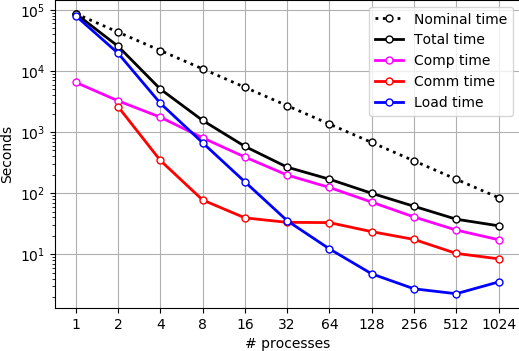
\includegraphics[width=\columnwidth]{figs/syntheticplot.png}
    \caption{Run times with the grid-like network.}
    \label{fig:mpirun}
\end{figure}


Figure \ref{fig:mpirun} shows the decomposition of the total simulation time into its three components: load time, communication time, and computation time. It also shows the `nominal' run time, which equals the serial total run time (with $n=1$) divided by the number of processes ($n$). This is the execution time that would be achieved if, for example, a simulation with 4 processes took one quarter of the time taken by the serial run. Such inversely proportional improvement is represented by a  straight line with negative unit slope in the log-log plot. Notice that the computation time indeed decreases at approximately this rate. However, the load time decreases at a rate that is approximately proportional to $1/n^2$ for $n\leq 32$. This is likely due to the large amount of memory required to store the network. The rate of improvement of the load time diminishes for $n \in[64, 512]$ and eventually worsens for $n>512$. This is due to the overhead involved in reading the network files. It can be seen then that the total simulation time is dominated by the load time for small values of $n$ ($n\leq 8$), which leads to super nominal (better than inversely proportional) improvements. For larger $n$ ($n\geq 16$), the total time is dominated by the computation time, which leads to inversely proportional improvements. For very large $n$ ($n\geq 512)$, the communication time begins to be significant, although it remains at about on tenth of the total simulation time for $n=1024$. The total simulation time was reduced by a factor of about 2,800 with $n=1024$, and could be further reduced with larger values. 

% The lower plot focuses on the simulations that are not distinguishable in the upper plot ($n\geq 6$). The trend is similar as in the first example, with inverse proportionality between the simulation time and the number of processes. 

% \begin{figure}[!ht]
%     \centering
%     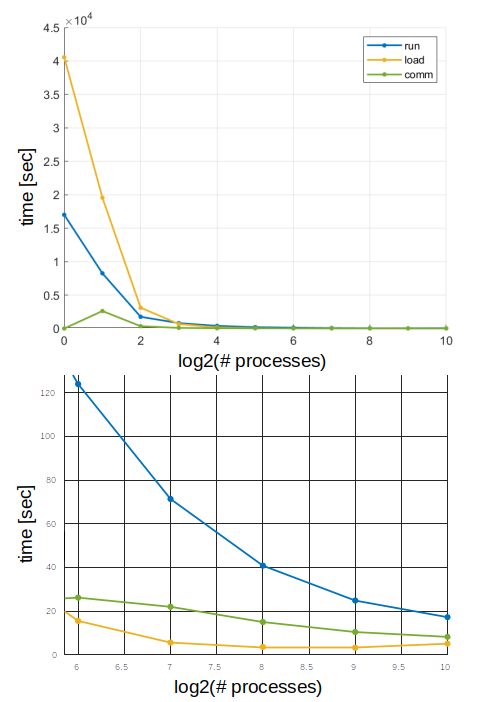
\includegraphics[width=\columnwidth]{figs/synthetic_results.png}
%     \caption{Parallel run times of the three phases of the algorithm with the grid-like network.}
%     \label{fig:mpirun}
% \end{figure}

% Figure~\ref{fig:scaling} demonstrate the scaling of OTM-MPI compared to the ideal scaling simulation rate. For each simulation experiment, the simulation rate $1/(simulation \:time)$, which corresponds to the number of simulations that can be completed within 1 seconds (simulations/s). The ideal rate is calculated as $(number\: of\: processes)*(serial\: simulation\: rate)$, and assumes that simulation rate increases proportionally with the number of processes. In practice, parallel simulation does not attain the ideal scaling rate as the $(communication\:time)/(simulation\:time)$ ratio grows with the number of processes. In fact, we observed that for the experiment with 1024 processes, each process spend half of its computation time in communicating with other processes. However, we still observed that for the simulation time, the parallel OTM had a speed up of 475 times with 1024 processes compared to the serial OTM. This corresponded to a time reduction from 8,245 seconds to 17 seconds.

% \begin{figure}[!ht]
%     \centering
%     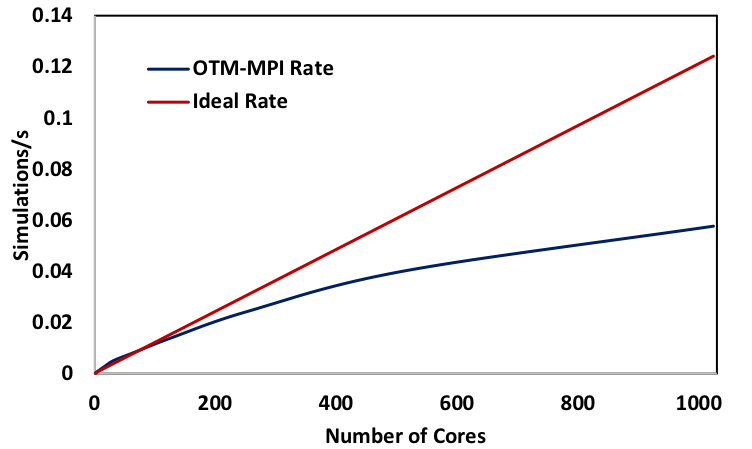
\includegraphics[width=\columnwidth]{figs/Scaling.png}
%     \caption{OTM scaling  compared to ideal scaling for the grid network.}
%     \label{fig:scaling}
% \end{figure}



\section{Conclusion}
The main contribution of this work is an open-source implementation of macroscopic traffic simulation for high-performance computing (HPC). As was detailed in the introduction, there are currently a host of platforms for running vehicle-based simulations in HPC. OTM-MPI offers an alternative for scenarios in which macroscopic modeling may be preferred over vehicle-based simulation. This may be the case if the following two conditions are given. First, that the available data is better suited for estimating macroscopic quantities (capacities) than microscopic ones (car-following rules). For example, if the data consists in loop detector measurements, and detailed vehicle accelerations are absent. Second, that the metrics of interest can be obtained from the macroscopic model. For instance, if we are interested in travel times and delays, and not in vehicle accelerations. Studies of routing behaviors in particular, either `natural' or induced by routing apps, can equally be carried out in macroscopic models. OTM-MPI can be obtained from \cite{otmmpi}.

\section*{Acknowledgement}
This work was supported in part by the Office of Science of
the U.S. Department of Energy under contract No. DE-AC02-
05CH11231. This work was authored in part by the National Renewable Energy Laboratory, operated by Alliance for Sustainable Energy, LLC, for the U.S. Department of Energy under Contract No. DE-AC36-08GO28308. 
% Funding provided by DOE's office of energy efficiency & renewable energy.



% \input{_bios}

\bibliography{_refs}{}
\bibliographystyle{IEEEtran}

\end{document}


